\documentclass[10pt, aspectratio=169]{beamer}

% === PAQUETES ===
\usepackage[utf8]{inputenc}
\usepackage[spanish]{babel}
\usepackage{amsmath, amssymb}
\usepackage{graphicx}
\usepackage{xcolor}
\usepackage{tikz}
\usepackage{listings}

% === RUTAS ===
\graphicspath{{figures/}}

% === TEMA Y COLORES ===
\usetheme{Madrid}
\usecolortheme{default}

% --- Paleta de Colores Personalizada (Trabajos de Grado) ---
% Colores Primarios
\definecolor{ColorVerdeOliva}{HTML}{636F03}   % Énfasis principal / Bullets
\definecolor{ColorNegroTex}{HTML}{1A171B}     % Texto principal
\definecolor{ColorRojoVino}{HTML}{B11F16}     % Alertas críticas
\definecolor{ColorMostaza}{HTML}{ACAA00}      % Énfasis secundario
\definecolor{ColorCremaBg}{HTML}{F3E7CE}      % Fondos de bloques

% Colores Secundarios
\definecolor{ColorNaranja}{HTML}{E95D0F}      % Gráficos / Llamados
\definecolor{ColorAzulOsc}{HTML}{122253}      % Títulos de frames
\definecolor{ColorTurquesa}{HTML}{0B8689}     % Enlaces
\definecolor{ColorAzulMed}{HTML}{1472B8}      % Ilustraciones
\definecolor{ColorMorado}{HTML}{634998}       % Agrupaciones

% Aplicación de colores a elementos Beamer
\setbeamercolor{frametitle}{fg=ColorAzulOsc, bg=ColorCremaBg}
\setbeamercolor{title}{fg=ColorAzulOsc}
\setbeamercolor{section in toc}{fg=ColorVerdeOliva}
\setbeamercolor{itemize item}{fg=ColorVerdeOliva}
\setbeamercolor{itemize subitem}{fg=ColorVerdeOliva}
\setbeamercolor{structure}{fg=ColorAzulOsc}
\setbeamercolor{normal text}{fg=ColorNegroTex}
\setbeamercolor{alerted text}{fg=ColorRojoVino}
\setbeamercolor{block title}{bg=ColorVerdeOliva, fg=white}
\setbeamercolor{block body}{bg=ColorCremaBg, fg=ColorNegroTex}

% === INFORMACIÓN DEL DOCUMENTO ===
\title{Modelado de Procesos Oceanográficos en el Caribe\\con Redes Neuronales Informadas por Física (PINN)}
\author{Autor}
\institute{Universidad}
\date{\today}

% === CONFIGURACIÓN DE TIEMPO ===
% Duración total estimada: 30 minutos
% Número de diapositivas: 18-24

\begin{document}

% Portada
\frame{\titlepage}

% Tabla de contenidos
\frame{\tableofcontents}

% === SECCIONES ===

\section{Introducción}
\begin{frame}[fragile]
  \frametitle{Introducción}
  
  \begin{block}{El desafío de la predicción atmosférica}
    La atmósfera es un sistema caótico gobernado por ecuaciones no lineales, donde pequeñas variaciones generan divergencias significativas (\emph{efecto mariposa}).
  \end{block}
  
  \begin{itemize}
    \item Nuevas fuentes de datos masivos: satélites, boyas, radares (ERA5, GOES)
    \item Limitación: métodos tradicionales requieren alto costo computacional
    \item Oportunidad: Redes Neuronales Físicamente Informadas (PINNs)
  \end{itemize}
  
  \note[item]{Contexto: clima predecible desde Babilonia hasta hoy; desafío de sistemas caóticos}
  \note[item]{Tiempo estimado: 2-3 minutos}
\end{frame}


\section{Planteamiento del Problema}
\begin{frame}[fragile]
  \frametitle{Planteamiento del Problema}
  
  \begin{alertblock}{El problema en la región Caribe}
    18 estaciones meteorológicas distribuidas en 404,7 km × 252,2 km\\
    \textbf{Densidad:} 1,8 estaciones por 10.000 km² $\Rightarrow$ insuficiente
  \end{alertblock}
  
  \begin{itemize}
    \small
    \item Datos dispersos no describen el estado continuo
    \item Vacíos de información en zonas sin instrumentación
    \item Necesidad de estimar presión y viento
  \end{itemize}
  
  \note[item]{Pregunta: ¿Cómo reconstruir campos atmosféricos desde datos dispersos?}
  \note[item]{Tiempo: 2-3 minutos}
\end{frame}

\begin{frame}[fragile]
  \frametitle{Planteamiento del Problema: Distribución de Estaciones}

  \begin{center}
    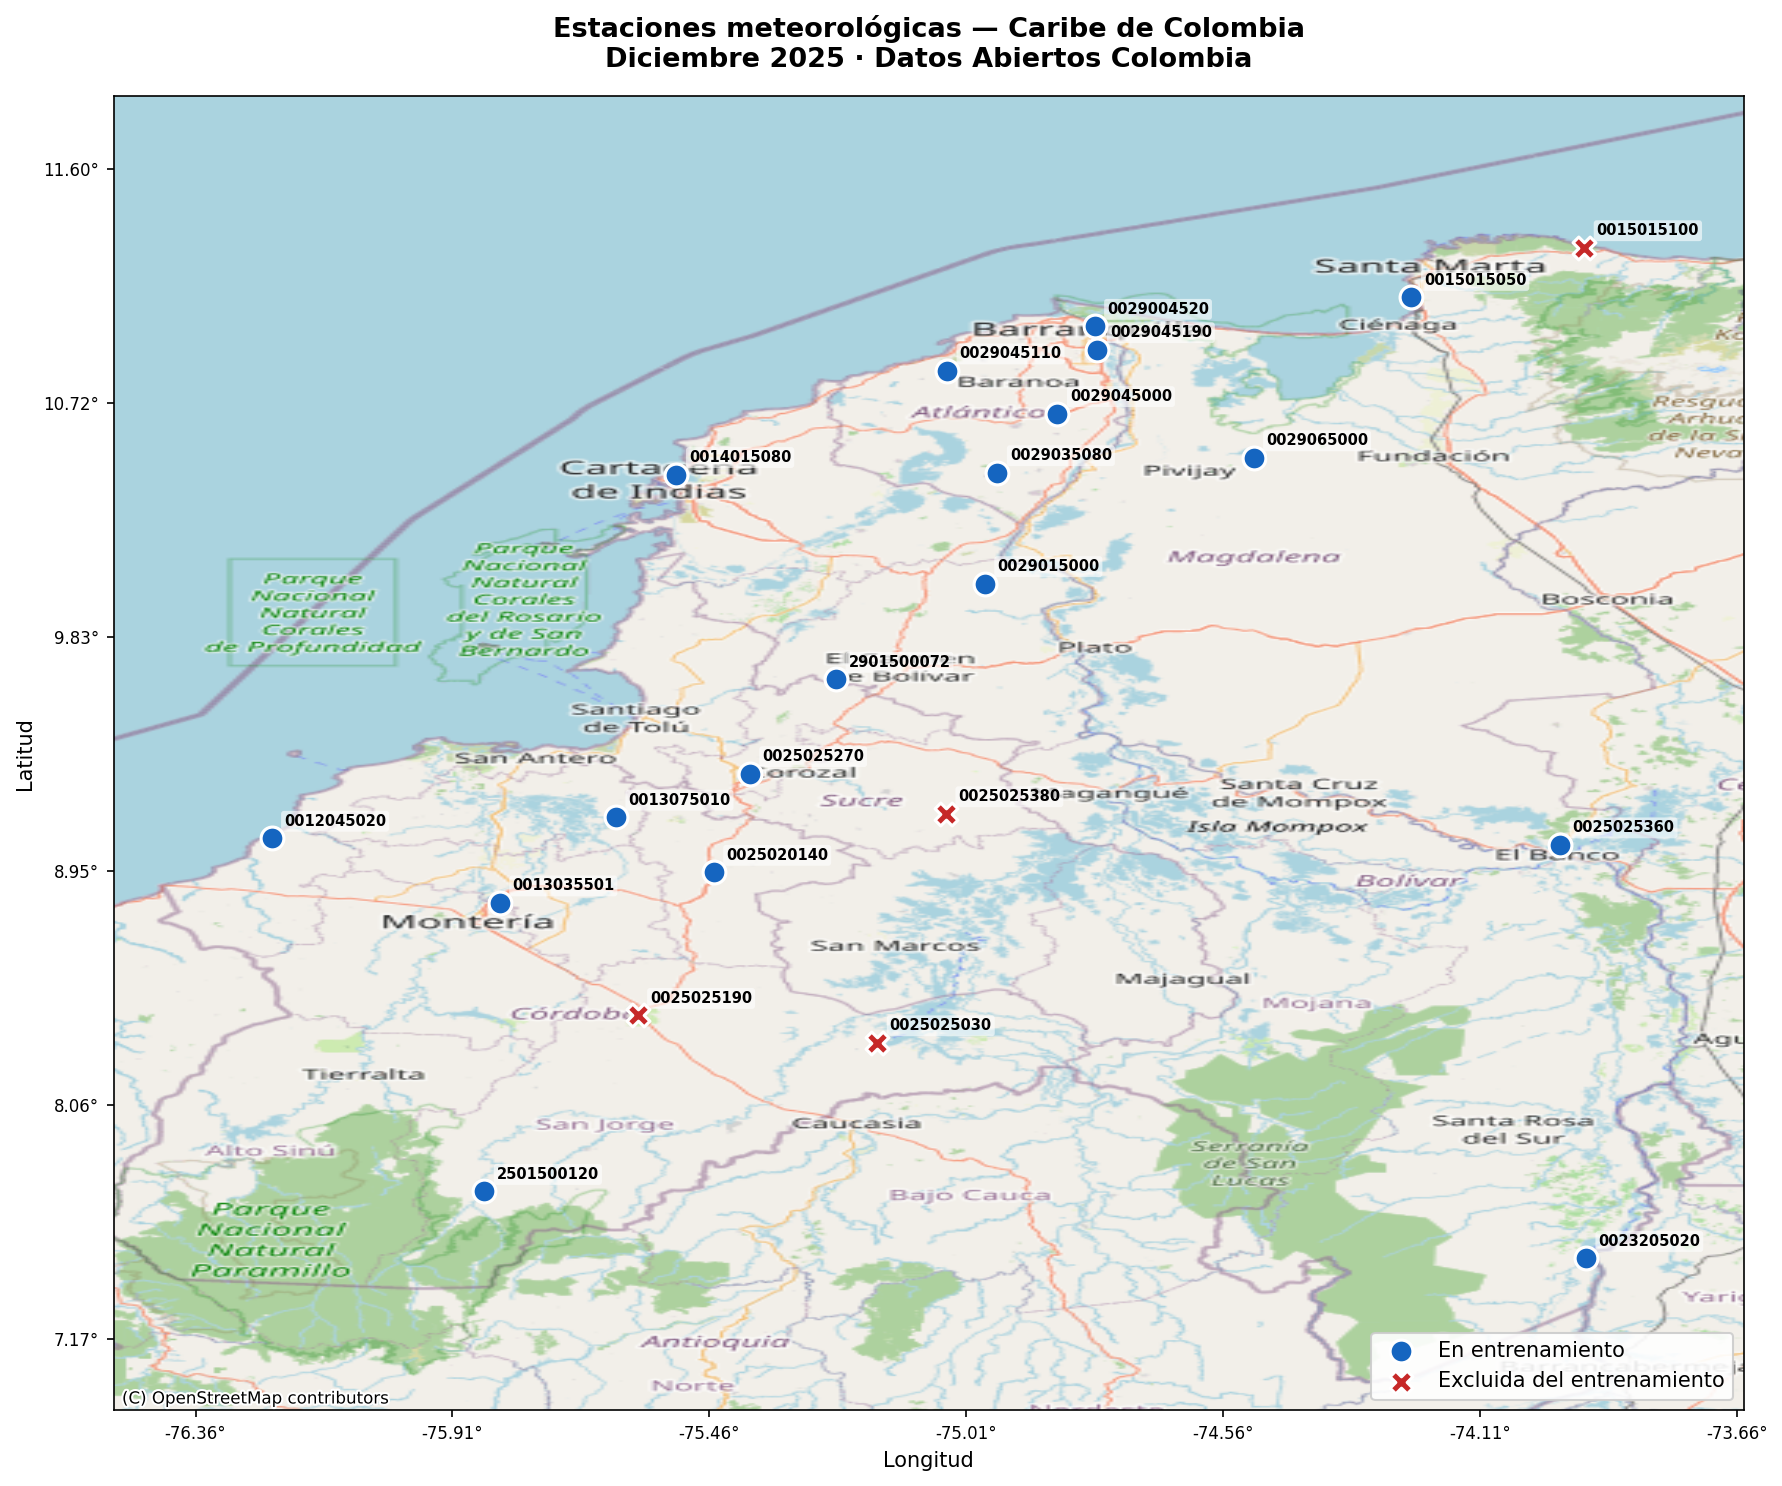
\includegraphics[width=0.85\textwidth]{figures/mapa_estaciones_caribe.png}
  \end{center}

  \note[item]{Mapa de cobertura espacial de las 18 estaciones meteorológicas en la región Caribe.}
\end{frame}

\begin{frame}[fragile]
  \frametitle{Pregunta de Investigación}

  \begin{block}{Pregunta central}
    \centering
    \large
    ¿Cómo construir un modelo basado en PINNs que, a partir de registros meteorológicos dispersos y de las ecuaciones de Navier-Stokes, permita estimar la presión y las componentes del viento sobre una malla espacio-temporal en puntos donde no existen estaciones de medición?
  \end{block}

  \note[item]{Conectar el problema de cobertura espacial con la necesidad de un modelo físicamente consistente.}
\end{frame}


\section{Objetivos}
\begin{frame}[fragile]
  \frametitle{Objetivos}
  
  \begin{block}{Objetivo General}
    Desarrollar una PINN basada en ecuaciones de Navier-Stokes y registros de estaciones meteorológicas para estimar presión y componentes del viento sobre una malla espacio-temporal en el litoral Caribe.
  \end{block}
  
  \begin{block}{Objetivos Específicos}
    \begin{enumerate}
      \item \textcolor{ColorVerdeOliva}{Organizar y preprocesar} datos de estaciones del IDEAM (diciembre 2025)
      \item \textcolor{ColorVerdeOliva}{Diseñar una PINN} que incorpore restricciones de N-S en su función de pérdida
      \item \textcolor{ColorVerdeOliva}{Evaluar desempeño} mediante métricas estándar (\alert{RMSE, MAE, $R^2$}) en datos de prueba
    \end{enumerate}
  \end{block}
  
  \note[item]{Tiempo estimado: 2-3 minutos}
\end{frame}


\section{Antecedentes}
\begin{frame}[fragile,shrink=5]
  \frametitle{Antecedentes: Métodos Tradicionales}
  
  \begin{block}{Modelos Numéricos (NWP)}
    Resuelven Navier-Stokes en mallas de alta resolución ($\sim$9 km).
    \begin{itemize}
      \item Costo: 2.5 millones horas CPU/día (ECMWF)
      \item Ventana: predicción $\approx$ 10 días (sensibilidad caótica)
      \item Limitación: necesita condiciones iniciales altamente precisas
    \end{itemize}
  \end{block}
  
  \begin{block}{Métodos Estadísticos}
    ARIMA, Procesos Gaussianos
    \begin{itemize}
      \item \textcolor{ColorVerdeOliva}{✓ Eficaces a corto plazo ($<$72 horas)}
      \item \textcolor{ColorRojoVino}{✗ Desconectados de física fundamental}
      \item \textcolor{ColorRojoVino}{✗ Fallan ante eventos extremos sin precedentes}
    \end{itemize}
  \end{block}
  
  \note[item]{Tiempo: 2 minutos}
\end{frame}

\begin{frame}[fragile]
  \frametitle{Antecedentes: Enfoques Modernos}
  
  \begin{block}{Machine Learning Convencional (GraphCast, FourCastNet)}
    \begin{itemize}
      \item \textcolor{ColorVerdeOliva}{✓ Rápidos: predicciones en minutos (vs. horas en NWP)}
      \item \textcolor{ColorVerdeOliva}{✓ Entrenados con décadas de datos ERA5}
      \item \textcolor{ColorRojoVino}{✗ Inconsistencias físicas: $\sim$5\% violación de energía}
      \item \textcolor{ColorRojoVino}{✗ Caja negra: imposible explicabilidad física}
    \end{itemize}
  \end{block}
  
  \begin{block}{Redes Neuronales Informadas por Física (PINNs)}
    Paradigma híbrido: celeridad del ML + rigor de EDP
    \begin{itemize}
      \item ✓ 30\% más precisión que NWP en casos críticos
      \item ✓ Garantiza coherencia física
      \item ✓ Requiere menos datos (conocimiento físico como regularizador)
    \end{itemize}
  \end{block}
  
  \note[item]{Tiempo: 2 minutos}
\end{frame}


\section{Marco Teórico}
\begin{frame}[fragile,shrink=5]
  \frametitle{Marco Teórico: Ecuaciones de Navier-Stokes}
  
  Conservación de momento y continuidad en fluidos viscosos:
  
  \begin{align*}
    \rho \left( \frac{\partial \mathbf{u}}{\partial t} + \mathbf{u} \cdot \nabla \mathbf{u} \right) &= -\nabla p + \mu \nabla^2 \mathbf{u} + \mathbf{f} \\
    \nabla \cdot \mathbf{u} &= 0
  \end{align*}
  
  Donde: $\mathbf{u}$ = velocidad, $p$ = presión, $\rho$ = densidad, $\mathbf{f}$ = fuerzas externas (Coriolis).
  
  \begin{block}{Reto clave}
    El término convectivo $(\mathbf{u} \cdot \nabla \mathbf{u})$ introduce no linealidad que dificulta soluciones analíticas.
  \end{block}
  
  \note[item]{Tiempo estimado: 3 minutos}
\end{frame}

\begin{frame}[fragile]
  \frametitle{PINNs: Redes Neuronales Informadas por Física}
  
  \begin{block}{Concepto clave}
    Las PINNs codifican ecuaciones diferenciales parciales directamente en su función de pérdida, garantizando que las predicciones respeten leyes físicas.
  \end{block}
  
  \begin{itemize}
    \item Combinan datos observados con restricciones físicas
    \item No requieren volúmenes masivos de datos
    \item Conocimiento físico actúa como regularizador
    \item 30\% más precisión que NWP en casos de intensificación rápida
  \end{itemize}
  
  \note[item]{Tiempo estimado: 2 minutos}
\end{frame}

\begin{frame}[fragile,shrink=8]
  \frametitle{Formulación: Función de Pérdida Híbrida}
  
  Una PINN minimiza una función de pérdida que combina dos términos:
  
  \begin{align*}
    \mathcal{L}_{total} = \mathcal{L}_{data} + \lambda \mathcal{L}_{physics}
  \end{align*}
  
  \begin{block}{Término de datos}
    \[\mathcal{L}_{data} = \frac{1}{N} \sum_{i=1}^{N} \left\| \hat{u}(x_i, y_i, t_i) - u^{obs}(x_i, y_i, t_i) \right\|^2\]
    Diferencia entre predicciones y observaciones de estaciones.
  \end{block}
  
  \begin{block}{Término físico}
    \[\mathcal{L}_{physics} = \frac{1}{M} \sum_{j=1}^{M} \left\| \text{NS}_{residual}(x_j, y_j, t_j) \right\|^2\]
    Residual de Navier-Stokes en malla de colocación (garantiza coherencia física).
  \end{block}
  
  \begin{alertblock}{Hiperparámetro crítico}
    $\lambda$ = peso del término físico (barrido: $\lambda \in \{1, 3, 5, 10\}$)
  \end{alertblock}
  
  \note[item]{Tiempo: 2 minutos}
\end{frame}


\section{Metodología}
\begin{frame}[fragile]
  \frametitle{Metodología: Datos y Dominio}
  
  \begin{block}{Datos de entrada}
    Estaciones meteorológicas IDEAM, región Caribe, diciembre 2025\\
    \textbf{Variables:} Lat/Long, tiempo, velocidad/dirección viento, presión, temperatura\\
    \textbf{Volumen:} 16.368 registros horarios de 22 estaciones (18 validadas)
  \end{block}
  
  \begin{block}{Dominio espacial}
    \begin{tabular}{ll}
      Latitud & 7,475° N a 11,115° N \\
      Longitud & 76,224° O a 73,926° O \\
      Extensión N-S & 404,7 km \\
      Extensión E-O & 252,2 km
    \end{tabular}
  \end{block}
  
  \note[item]{Tiempo estimado: 2-3 minutos}
\end{frame}

\begin{frame}[fragile]
  \frametitle{Metodología: Arquitectura de la PINN}
  
  \begin{block}{Estructura de la red neuronal}
    \begin{itemize}
      \item \textbf{12 capas} con \textbf{1.200 neuronas} cada una
      \item Capa personalizada \texttt{GammaBiasLayer}: Weight Normalization desacoplada
      \item Parámetros entrenables: $\approx$ 15,89 millones
      \item Entrada: $(x, y, t)$ normalizado | Salida: $(u_x, u_y, p)$ adimensional
    \end{itemize}
  \end{block}
  
  \begin{block}{Diseño y regularización}
    \begin{itemize}
      \item \textbf{8 capas Tanh} (no linealidad) + \textbf{4 capas Lineales} (regularización implícita)
      \item Pérdida física evaluada en 226.176 puntos de colocación (regularizador)
      \item Ratio parámetros/datos: 1.186:1 para 13.392 puntos de entrenamiento
    \end{itemize}
  \end{block}
  
  \note[item]{Tiempo estimado: 2-3 minutos}
\end{frame}

\begin{frame}[fragile]
  \frametitle{Metodología: Barrido de Hiperparámetros}
  
  \begin{block}{Configuración experimental}
    \begin{itemize}
      \item Epochs: 2.000
      \item Learning rate: $1 \times 10^{-4}$ con ReduceLROnPlateau
      \item Datos por estación: 300 registros (5.400 totales)
      \item Malla de colocación: 304 puntos ($R = 0{,}1°$) o 44 puntos ($R = 0{,}4°$)
    \end{itemize}
  \end{block}
  
  \begin{block}{Variables barridas}
    Resolución de malla $R \in \{0{,}1°, 0{,}4°\}$\\
    Peso físico $\lambda \in \{1, 3, 5, 10\}$
  \end{block}
  
  \note[item]{Tiempo estimado: 2-3 minutos}
\end{frame}


\section{Resultados}
% ===== FRAME 13: Tabla de Desempeño Comparativo (MANTENER) =====
\begin{frame}[fragile,shrink=10]
  \frametitle{Resultados: Desempeño Comparativo}
  
  \begin{block}{Mejor modelo: \texttt{todos\_R01\_L5}}
    Resolución $R = 0{,}1°$, $\textcolor{ColorVerdeOliva}{\lambda = 5}$, datos completos ($\sim$744 reg/est)
  \end{block}
  
  \scriptsize
  \begin{table}
    \centering
    \begin{tabular}{lcccccc}
      \hline
      Modelo & Loss & MSE$_{u_x}$ & MSE$_{u_y}$ & MSE$_p$ & $\mathcal{R}_{NS}$ \\
      \hline
      \textbf{\textcolor{ColorVerdeOliva}{todos\_R01\_L5}} & 0,9261 & 0,4633 & 0,4347 & 1,3688 & \textbf{\textcolor{ColorRojoVino}{0,01273}} \\
      300xest\_R01\_L5 & 1,1207 & 0,4689 & 0,4647 & 1,6220 & 0,03682 \\
      300xest\_R04\_L1 & 1,0575 & 0,5059 & 0,5085 & 1,5720 & 0,24141 \\
      300xest\_R01\_L1 & 1,1380 & 0,4806 & 0,4756 & 1,6477 & 0,20107 \\
      300xest\_R04\_L10 & 1,0859 & 0,5220 & 0,5224 & 1,6185 & 0,02242 \\
      300xest\_R01\_L10 & 1,1624 & 0,4919 & 0,4966 & 1,6906 & 0,02318 \\
      \hline
    \end{tabular}
  \end{table}
  
  \normalsize
  \begin{itemize}
    \item Error observacional promedio: \alert{0,7556} (mejor entre todos)
    \item Residual Navier-Stokes: \alert{0,01273} (máxima coherencia física)
  \end{itemize}
  
  \note[item]{Tiempo: 1,5 minutos}
\end{frame}

% ===== FRAME 14: Análisis de Convergencia (MANTENER) =====
\begin{frame}[fragile]
  \frametitle{Resultados: Análisis de Convergencia}
  
  \begin{block}{Ranking por error observacional promedio}
    \begin{enumerate}
      \small
      \item (1) todos\_R01\_L5: 0,7556 (coherencia física: 0,01273)
      \item (2) 300xest\_R01\_L5: 0,8187 (coherencia física: 0,03682)
      \item (3) 300xest\_R01\_L10: 0,8267 (coherencia física: 0,02318)
    \end{enumerate}
  \end{block}
  
  \begin{columns}[T]
    \column{0.5\textwidth}
    \centering
    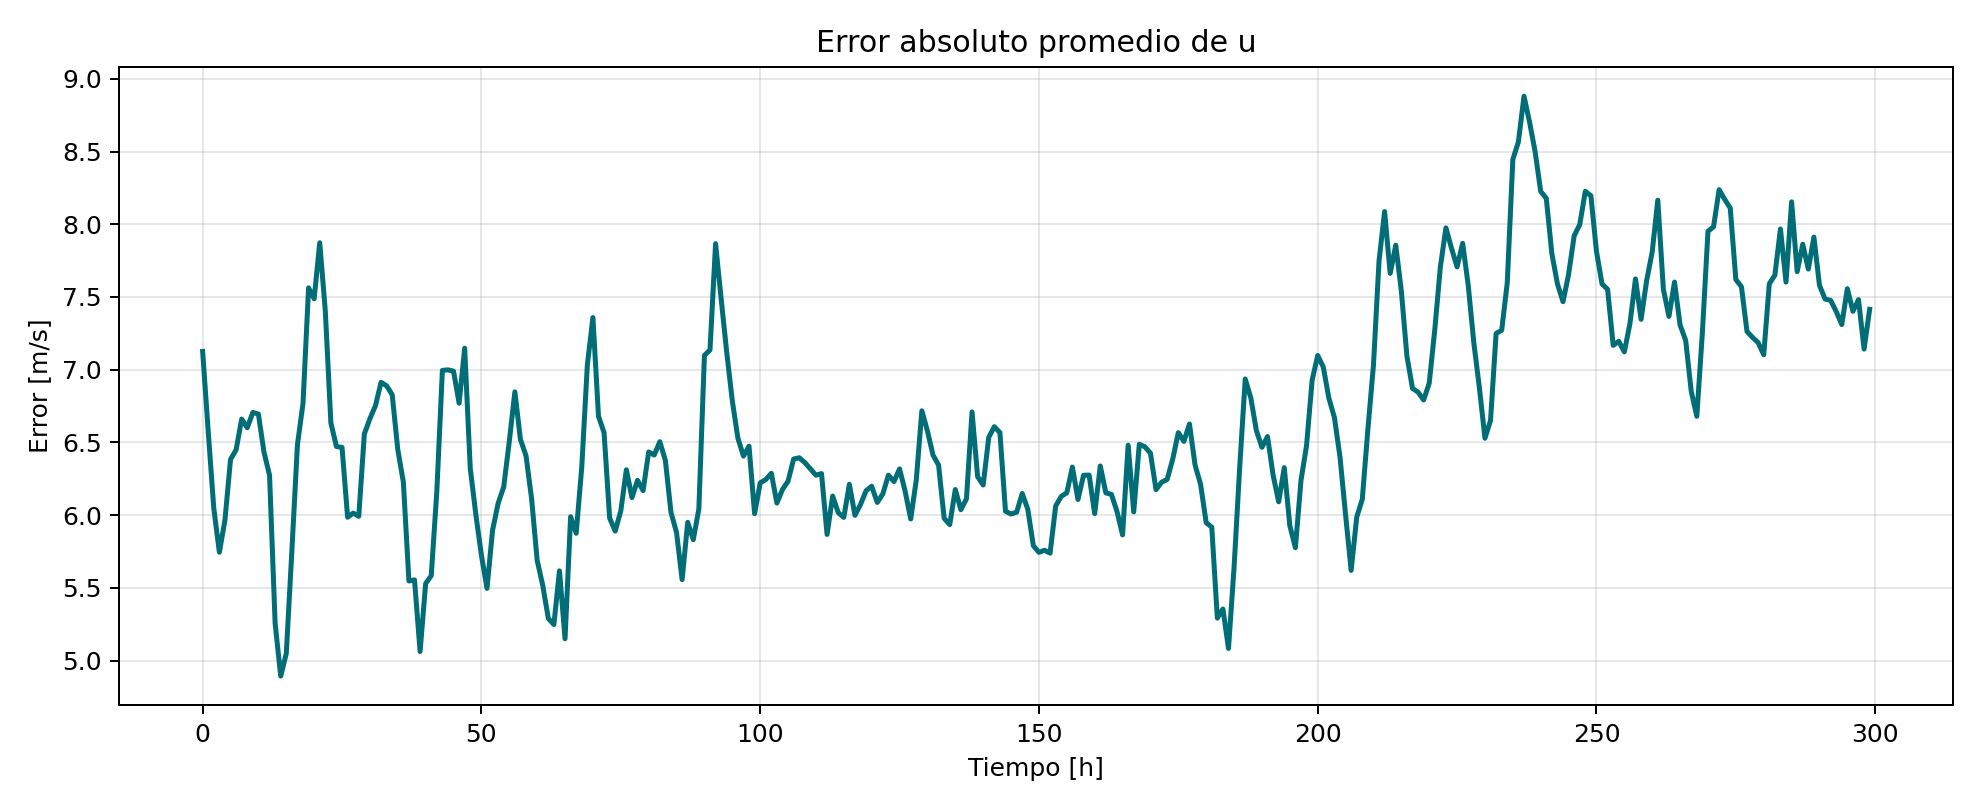
\includegraphics[width=\textwidth]{figures/error_u.png}
    \tiny Error promedio $u_x$ (m/s)
    
    \column{0.5\textwidth}
    \centering
    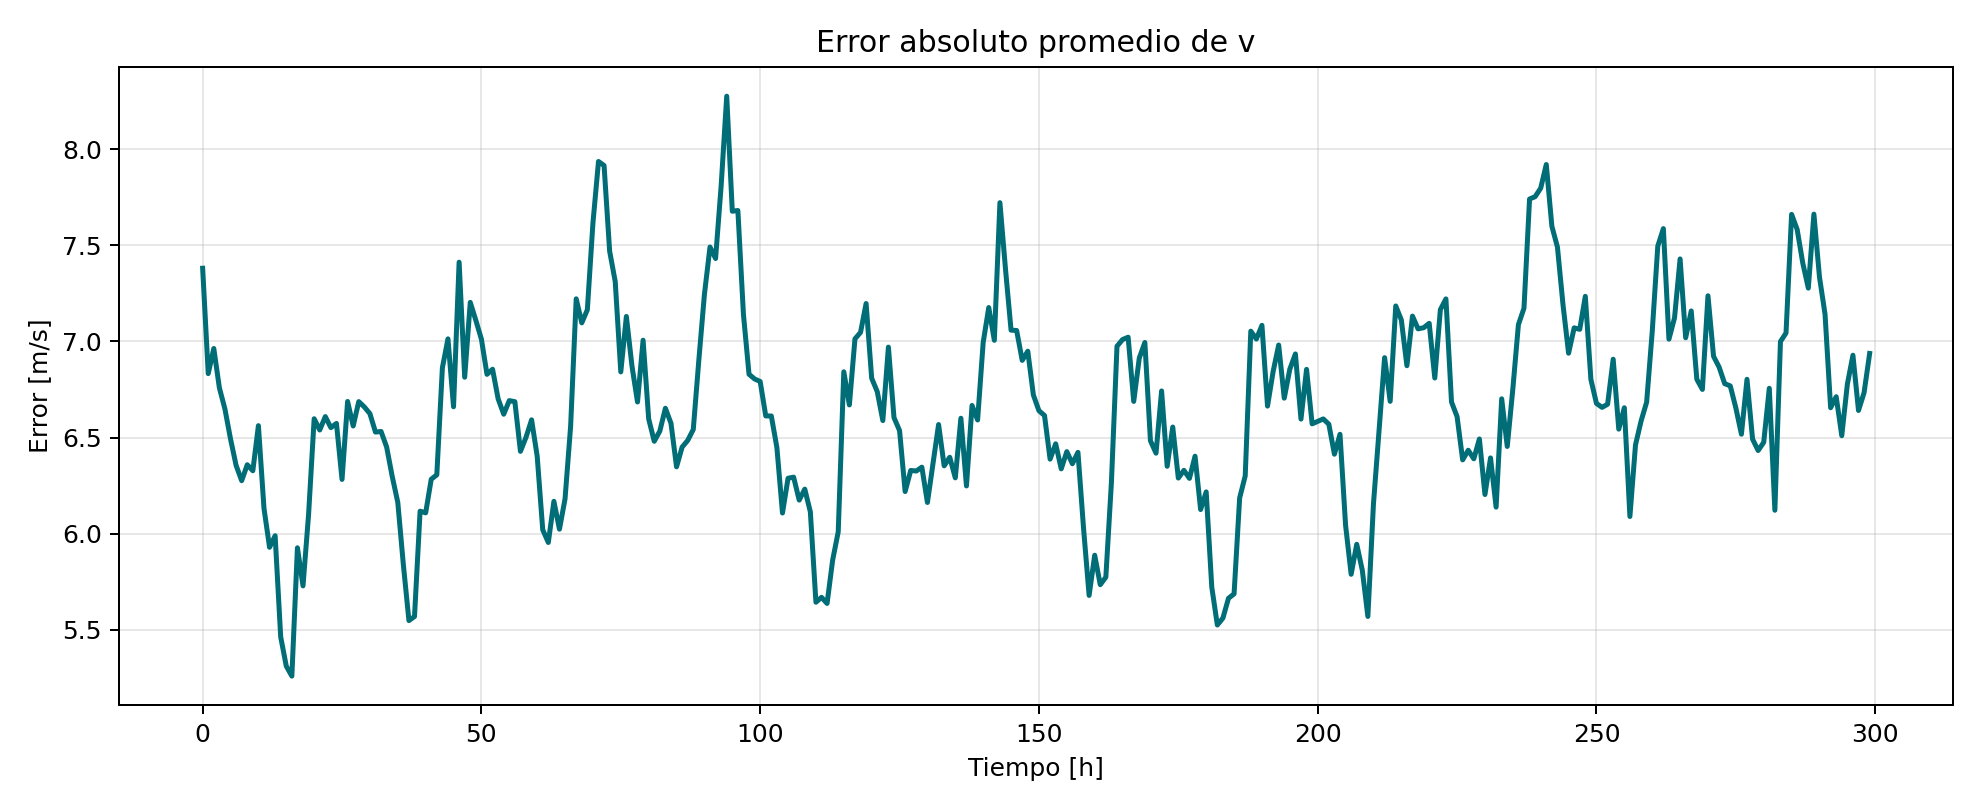
\includegraphics[width=\textwidth]{figures/error_v.png}
    \tiny Error promedio $u_y$ (m/s)
  \end{columns}
  
  \note[item]{Gráficos: Convergencia del error en componentes de viento}
  \note[item]{Tiempo: 1,5 minutos}
\end{frame}

% ===== FRAME 15: Validación Fuera de Muestra (NUEVA) =====
\begin{frame}[fragile,shrink=8]
  \frametitle{Resultados: Validación Fuera de Muestra}

  \begin{block}{Tabla 5.8: Comparación de métricas (train vs. test temporal)}
    \scriptsize
    \centering
    \begin{tabular}{lccc}
      \hline
      Métrica & Entrenamiento (días 1--20) & Prueba (días 21--31) & Diferencia \\
      \hline
      $\text{MSE}_{u_x}$ & 0{,}4633 & \textbf{0{,}4422} & $-4{,}5$\,\% \\
      $\text{MSE}_{u_y}$ & 0{,}4347 & \textbf{0{,}4248} & $-2{,}3$\,\% \\
      $\text{MSE}_{p}$   & 1{,}3688 & \textbf{3{,}9116} & $+185{,}8$\,\% \\
      $\mathcal{R}_{\text{NS}}$ & 0{,}01273 & \textbf{0{,}03640} & $+186{,}0$\,\% \\
      \hline
    \end{tabular}
  \end{block}

  \begin{block}{Lectura técnica}
    \begin{itemize}
      \small
      \item Generalización favorable en viento: $u_x$ y $u_y$ se mantienen estables en prueba.
      \item Brecha crítica en presión y residual físico: evidencia de dificultad de extrapolación temporal.
      \item Mensaje clave: buena robustez para velocidad, cautela para presión fuera del período de entrenamiento.
    \end{itemize}
  \end{block}

  \note[item]{Tiempo: 1,5 minutos}
  \note[item]{Fuente: Tabla 5.8 de la sección 5.5 (validación fuera de muestra)}
\end{frame}

% ===== FRAME 17: Análisis de Pérdida Total Comparativa (NUEVA) =====
\begin{frame}[fragile]
  \frametitle{Análisis: Comparativa de Pérdida Total}
  
  \begin{block}{Tabla 5.4: Comparación de resoluciones ($\overline{\text{MSE}}_{\text{obs}}$)}
    \scriptsize
    \centering
    \begin{tabular}{ccccc}
      \hline
      $\lambda$ & R=0,1 & R=0,4 & $\Delta$ (R0,4 - R0,1) & Mejor R \\
      \hline
      1  & 0,86796 & 0,86216 & -0,0058 & 0,4 \\
      3  & 1,24982 & 1,02208 & -0,2277 & 0,4 \\
      5  & 0,85185 & 1,32126 & +0,4694 & \textbf{0,1} \\
      10 & 0,89305 & 0,88765 & -0,0054 & 0,4 \\
      \hline
    \end{tabular}
  \end{block}

  \begin{block}{Lectura técnica}
    \begin{itemize}
      \small
      \item R=0,4 domina en $\lambda \in \{1,3,10\}$.
      \item El único caso donde la malla fina supera claramente es $\lambda = 5$.
      \item Decisión final: R=0,1 con $\lambda = 5$ por mejor equilibrio en el régimen óptimo.
    \end{itemize}
  \end{block}
  
  \note[item]{Tiempo: 1,5 minutos}
  \note[item]{Fuente: Tabla 5.4 (Comparación de resoluciones), doctg/18_resultados.tex}
\end{frame}

% ===== FRAME 18: Efecto de la Restricción Suave de Rango (NUEVA) =====
\begin{frame}[fragile]
  \frametitle{Resultados: Efecto de la Restricción Suave de Rango}

  \begin{block}{Tabla 5.6: Comparación de pérdida final (época 2.000)}
    \scriptsize
    \centering
    \begin{tabular}{lccc}
      \hline
      Experimento & Registros totales & Mecanismo de rango & Loss final \\
      \hline
      \texttt{300xest\_R01\_L5} & 5.400 & No & 1,117 \\
      \texttt{todos\_R01\_L5} & 13.392 & No & 0,926 \\
      \texttt{todosreg\_R01\_L5\_rangeL05} & 13.392 & Sí & \textbf{0,638} \\
      \hline
    \end{tabular}
  \end{block}

  \begin{block}{Lectura técnica (sección 5.4.6)}
    \begin{itemize}
      \small
      \item Manteniendo $R=0{,}1^\circ$ y $\lambda=5$, activar rango reduce la loss final de 0,926 a 0,638.
      \item Reducción relativa frente al modelo equivalente sin rango: \textbf{-31,1\%}.
      \item La restricción de rango regulariza la optimización y mejora la plausibilidad del campo previo a visualizar $u$ y $v$.
    \end{itemize}
  \end{block}

  \note[item]{Tiempo: 1,5 minutos}
  \note[item]{Transición: esta mejora en loss se evidencia espacialmente en los campos predichos de velocidad}
\end{frame}

% ===== FRAME 19: Campos Predichos de Velocidad (NUEVA) =====
\begin{frame}[fragile]
  \frametitle{Resultados: Campos Predichos de Velocidad}

  \begin{block}{Interpretación física de la mejor corrida con restricción de rango}
    La configuración \texttt{todosreg\_R01\_L5\_rangeL05} no solo reduce la pérdida total,
    sino que genera campos espaciales continuos y físicamente plausibles para las componentes
    horizontales del viento sobre el dominio Caribe.
  \end{block}

  \begin{columns}[T]
    \column{0.5\textwidth}
    \centering
    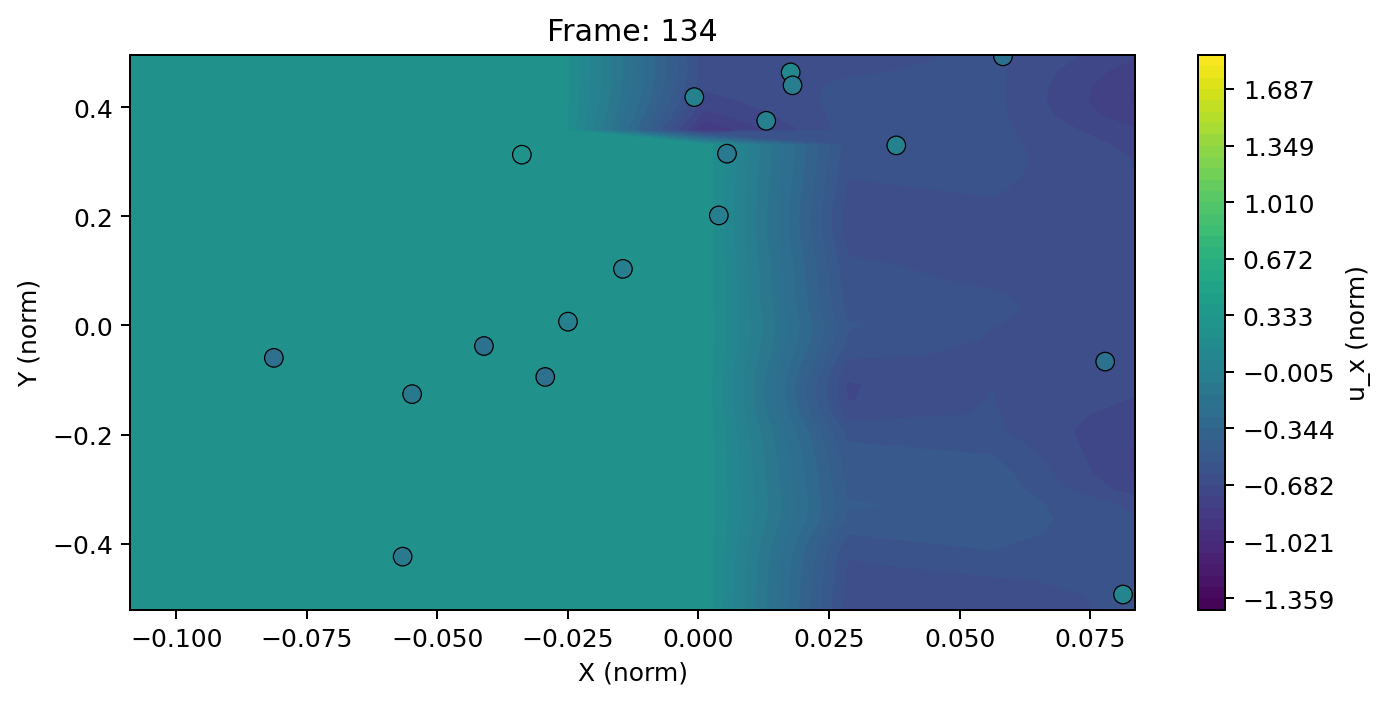
\includegraphics[width=\textwidth]{figures/pinn_campo_u_t134.png}
    \tiny Campo predicho final de $u$

    \column{0.5\textwidth}
    \centering
    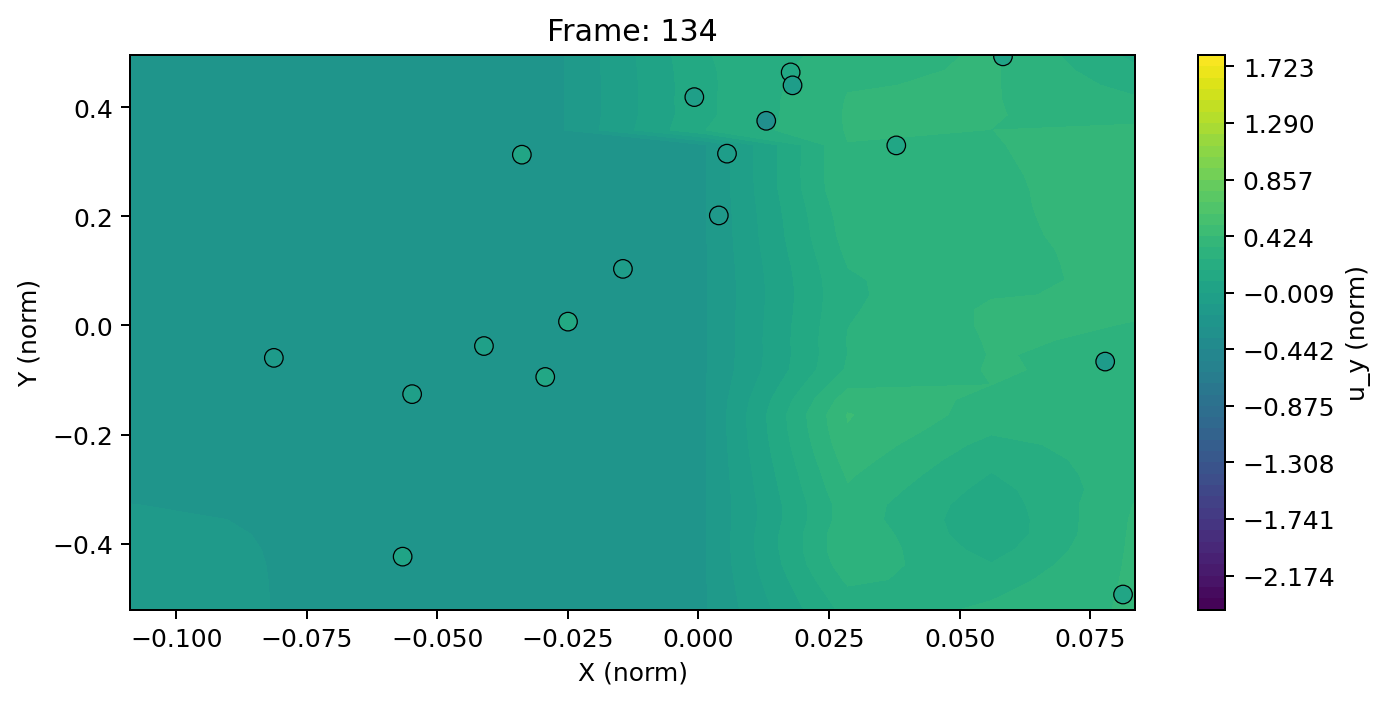
\includegraphics[width=\textwidth]{figures/pinn_campo_v_t134.png}
    \tiny Campo predicho final de $v$
  \end{columns}

  \note[item]{Tiempo: 1,5 minutos}
  \note[item]{Clave: traducir la mejora en pérdida a una evidencia espacial interpretable}
\end{frame}


\section{Discusión}
\begin{frame}[fragile]
  \frametitle{Discusión}
  
  \begin{block}{Logros principales}
    \begin{itemize}
      \item Integración exitosa de N-S con datos dispersos: $\mathcal{R}_{NS} = 0{,}01273$
      \item Menor dependencia de datos: 300 muestras por estación vs. millones de datos en ML convencional
      \item Coherencia física garantizada en extrapolación
    \end{itemize}
  \end{block}
  
  \begin{block}{Ventaja vs. métodos alternativos}
    \textbf{vs. NWP:} 30\% menor costo computacional, no requiere condiciones iniciales altamente precisas\\
    \textbf{vs. Estadísticos:} Respeta leyes físicas, válido en eventos extremos\\
    \textbf{vs. ML puro:} Errores físicos reducidos, generalización mejorada
  \end{block}
  
  \note[item]{Tiempo estimado: 3 minutos}
\end{frame}


\section{Conclusiones}
\begin{frame}[fragile]
  \frametitle{Conclusiones}
  
  \begin{block}{Contribuciones principales}
    \begin{itemize}
      \item Demostración exitosa de PINNs en reconstrucción meteorológica a escala local
      \item Metodología reproducible y escalable para regiones con datos dispersos
      \item Validación de coherencia física ($\mathcal{R}_{NS} = 0,01273$) en modelos híbridos
    \end{itemize}
  \end{block}
  
  \begin{block}{Logro de objetivos}
    [Org] Organización y preprocesamiento: 16.368 registros de 18 estaciones\\
    [Diseño] Diseño e implementación: PINN con restricciones N-S integradas\\
    [Eval] Evaluación: 9 experimentos con métricas reproducibles
  \end{block}
  
  \note[item]{Tiempo: 2 minutos}
\end{frame}

\begin{frame}[fragile]
  \frametitle{Trabajo Futuro}
  
  \begin{block}{Extensiones inmediatas}
    \begin{itemize}
      \item Predicción temporal: transición de interpolación a pronóstico ($t + \Delta t$)
      \item Incorporación de variables adicionales: humedad relativa, radiación solar
      \item Análisis de sensibilidad a resolución de malla ($R$ más fina)
    \end{itemize}
  \end{block}
  
  \begin{block}{Aplicaciones emergentes}
    \begin{itemize}
      \item Extensión a otras regiones oceanográficas (Pacífico colombiano, cuencas andinas)
      \item Acoplamiento con modelos de dispersión de contaminantes
      \item Integración en sistemas operativos de monitoreo ambiental
    \end{itemize}
  \end{block}
  
  \note[item]{Tiempo: 1,5 minutos}
\end{frame}

\begin{frame}[plain,c]
  \centering
  \huge{Gracias}
  \note[item]{Cierre (0,5 min)}
\end{frame}


\end{document}
